%%%%%%%%%%%%%%%%%%%%%%%%%%%%%%%%%%%%%%%%%%%%%%%%%%%%%%%%%%%%%%%%%%%%%%%%%%%%%%%%
% Copyright 2019-2022 Louis Paternault --- http://snt.ababsurdo.fr
%
% Publié sous licence Creative Commons Attribution-ShareAlike 4.0 International (CC BY-SA 4.0)
% http://creativecommons.org/licenses/by-sa/4.0/deed.fr
%%%%%%%%%%%%%%%%%%%%%%%%%%%%%%%%%%%%%%%%%%%%%%%%%%%%%%%%%%%%%%%%%%%%%%%%%%%%%%%%

% Pour compiler :
%$ lualatex $basename

\documentclass[11pt]{article}

\usepackage{2223-pablo}
\usepackage{2223-pablo-paternault}
\usepackage[
  a5paper,
  margin=5mm,
  includehead,
  headsep=3mm,
]{geometry}
\usepackage{2223-pablo-header}
\fancyhead[L]{\textsc{SNT > Le Web}}
\fancyhead[R]{\textsc{Algorithme \emph{page rank}}}

\usepackage{2223-pablo-tikz}
\usepackage{multicol}

\begin{document}

%Lorsqu'une personne fait une requête sur un moteur de recherche, celui-ci affiche une liste de pages correspondantes, en présentant les pages les plus populaires en premier. Comment fait ce moteur de recherche pour déterminer les pages les plus populaires ?
%
%Dans cette activité, nous allons présenter une version simplifiée de l'algorithme \emph{PageRank}, inventé par Larry Page (confondateur de Google).
%
%\subsubsection*{Présentation de l'algorithme}
%
%La plupart des pages web présentent des liens vers d'autres pages web, appelés liens hypertextes. Le principe général est que si une page web est beaucoup référencée par les autres pages web, cette page est plus importante, et sera bien classée par les moteurs de recherche (ceci sera affiné plus tard).
%
%Pour mesurer cette popularité par un nombre, on applique l'algorithme suivant :
%\begin{itemize}
%  \item on part d'une page web au hasard (on suppose que cela n'a pas d'importance, ce qui es partiellement vrai) ;
%  \item sur chaque page visitée, on :
%      clique sur un lien au hasard sur cette page (pour visiter une nouvelle page) ;
%    \item on répète cette étape un grand nombre de fois.
%\end{itemize}
%Durant l'exécution de l'algorithme, on n'oublie pas de compter le nombre de fois que chaque page a été visitée. Le score de chaque page est alors la fréquence du nombre de visites de cette page. Les pages avec le plus haut score seront visitées plus souvent que les autres.

\subsubsection*{Exemple}

\begin{multicols}{2}
Le graphe suivant représente un ensemble de page web, nommées A à G. Les arêtes (flèches) représentent des liens entre les pages. Par exemple, il y a une arête allant de la page B à la page G, ce qui signifie qu'il est possible, en visitant la page B, de cliquer sur un lien pour se retrouver sur la page G.

En vous mettant par deux, en simulant le lancer d'un dé à six face avec votre calculatrice, parcourez aléatoirement ces pages web, en notant bien le nombre de visites. %Pour cela, par binôme, pendant quelques minutes, en partant d'un sommet choisi au hasard :

\columnbreak

\begin{center}
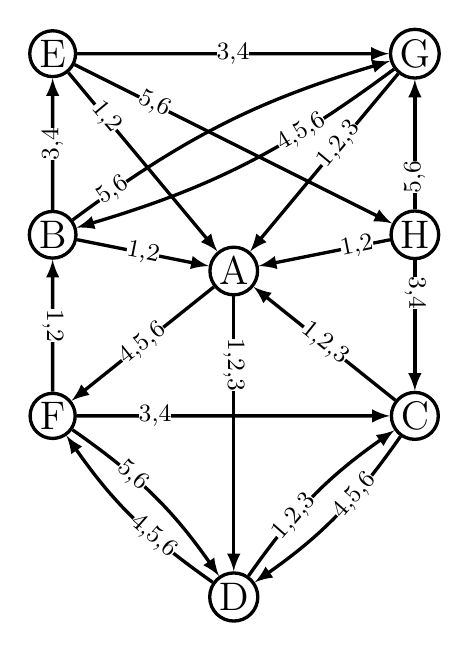
\begin{tikzpicture}[scale=2.3, very thick]
  \tikzstyle{sommet}=[circle, draw, minimum size=1em, inner sep=1, font=\Large];
  \tikzstyle{arete}=[-latex];
  \tikzstyle{proba}=[near start, sloped, fill=white, font=\small, inner sep=0];

  \node[sommet] (A) at (0, -.2) {A};
  \node[sommet] (B) at (-1, 0) {B};
  \node[sommet] (C) at (1, -1) {C};
  \node[sommet] (D) at (0, -2) {D};
  \node[sommet] (E) at (-1, 1) {E};
  \node[sommet] (F) at (-1, -1) {F};
  \node[sommet] (G) at (1, 1) {G};
  \node[sommet] (H) at (1, 0) {H};

  \draw[arete] (A) -- (D) node[proba]{1,2,3};
  \draw[arete] (A) -- (F) node[proba, midway]{4,5,6};
  \draw[arete] (B) -- (A) node[proba, midway]{1,2};
  \draw[arete] (B) -- (E) node[proba, midway]{3,4};
  \draw[arete] (B) edge[bend left=10] node[proba, very near start]{5,6} (G);
  \draw[arete] (C) -- (A) node[proba, midway]{1,2,3};
  \draw[arete] (C) edge[bend left=10] node[proba, pos=.35]{4,5,6} (D);
  \draw[arete] (D) edge[bend left=10] node[proba, pos=.35]{1,2,3} (C);
  \draw[arete] (D) edge[bend left=10] node[proba, pos=.35]{4,5,6} (F);
  \draw[arete] (E) -- (A) node[proba]{1,2};
  \draw[arete] (E) -- (G) node[proba, midway]{3,4};
  \draw[arete] (E) -- (H) node[proba]{5,6};
  \draw[arete] (F) -- (B) node[proba, midway]{1,2};
  \draw[arete] (F) -- (C) node[proba]{3,4};
  \draw[arete] (F) edge[bend left=10] node[proba, pos=.35]{5,6} (D);
  \draw[arete] (G) -- (A) node[proba, pos=.4]{1,2,3};
  \draw[arete] (G) edge[bend left=10] node[proba, pos=.3]{4,5,6} (B);
  \draw[arete] (H) -- (A) node[proba, proba]{1,2};
  \draw[arete] (H) -- (C) node[proba, proba]{3,4};
  \draw[arete] (H) -- (G) node[proba, proba]{5,6};
\end{tikzpicture}
\end{center}
\end{multicols}

% \begin{itemize}
%   \item un élève lance un dé encore et encore ;
%   \item l'autre élève suit le chemin parcouru, en se déplaçant sur le graphe en suivant le résultat du dé.
% \end{itemize}

Lorsque vous avez fait 50 déplacement (environ),  venez écrire les résultats trouvés sur l'ordinateur du professeur.

\subsubsection*{Analyse}

\begin{enumerate}
  \item Reportez sur le graphe plus haut les scores \emph{PageRank} calculés avec la classe.
      \item Comptez, pour chaque page, le nombre de liens qui proviennent d'autres pages.
    \end{enumerate}
    On s'intéresse à l'affirmation :
    \emph{\og Plus une page a de liens qui viennent \emph{vers} elle, plus son score \emph{PageRank} est élevé.\fg}
    \begin{enumerate}
        \setcounter{enumi}{2}
      \item En comparant les pages A, G, H, cette affirmation vous semble-t-elle correcte ?
      \item En comparant les pages A et D, cette affirmation vous semble-t-elle correcte ? Comment expliquer cela ?
\end{enumerate}

\subsubsection*{\emph{Search Engine Optimization}}

Vous êtes l'auteur de la page H, et vous voulez augmenter votre score \emph{PageRank}. En vous servant des réponses aux questions précédentes, imaginez un moyen pour augmenter artificiellement votre score (en créant de nouveaux liens \emph{depuis la page F}, ou depuis de nouvelles pages que vous créez).

\end{document}
